\chapter{Introduction}

The increase of computaional power enabled the integration of deep learning concepts in real-world scenarios.
Training of large datasets for supervised learning models leads to a lot of problem solvers and automation in business and private areas of society.
The technology influences a large amount of people every day with rising tendency.
Well-known uses are algorithms for search, personalized adds, voice assistants, autonomous vehicles, transportation and network security.
\hfill \break
Scientist with technical knowledge integrade the concepts of deep learning into nearly every industry and branch.
Great examples for current real-world easements are in healthcare, marketing and agriculture:

IBM develops software that supports diagnosing, treating and predicting outcomes in medical situations.
Their deep learning algorithms have the ability to read and filter unstructured data, find similarities between patients and finding information in medical literature that helps to discover new insights.
Doctors benefit from personalized patient treatment plans and better analysis by the monitoring of patients. Researchers can discover new insights in drug development.
Currently the IBM Watson Healthcare software helps more than 230 healthcare organizations worldwide with more than 15,000 clients and partners. Their cognitive offerings have impacted care or social services for more than 295,000 people.
\cite{ibm-watson-healthcare, ibm-watson-facts}

Airbnb, a online marketplace for renting homes uses deep neural networks for categorising its listing photos.
The decision of their customers is influenced by a diverse set of images.
Many home providers label their images wrong and have not enough variety in their collection.
Moreover their total amount of photos is nearly half a billion images.
Deep learning helps them identifying the picture and presenting them on the site properly.
Moreover they can detect certain objects in the images, which enable custom filters and searches for objects.
\cite{airbnb-ic-video, airbnb-ic-blog}

\begin{figure}[H]
    \centering
    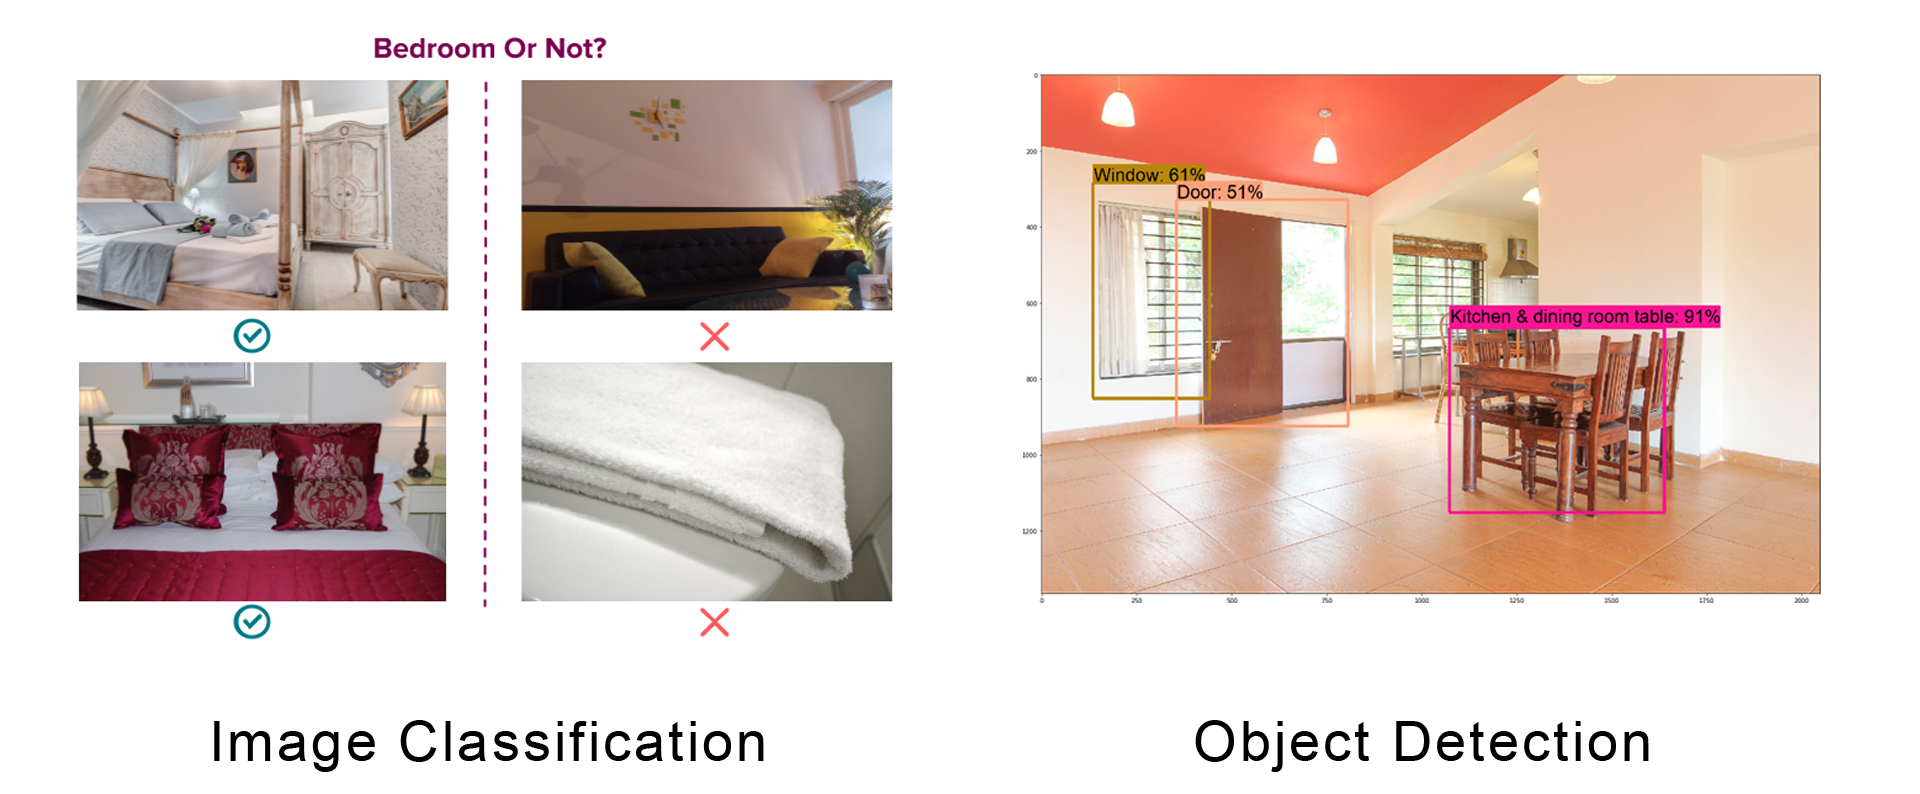
\includegraphics[width=\textwidth]{airbnb_classification_and_detection}
    \caption{\cite{airbnb_image_classification, airbnb_object_detection} Airbnb image classification and object detection}
    \label{fig:airbnb_image_classification}
\end{figure}

Connecterra developed an intelligent dairy farmer assistant.
They discovered that the production of milk is based on the animal’s health.
With an animal observation and machine learning they are able to diagnose problems early and provide health recommandations to the farmers.
\cite{tensorflow-stories, connecterra-video, connecterra-web}

The latest outstanding milestone in research: An AI algorithm developed by Google DeepMind had beaten two of the worls's best StarCraft 2 players.
StarCraft, a Real-Time Strategy (RTS) game was called the "grand challenge" for AI because of the game complexity.
To win in this game the algorithm needs to develop continually new frontiers of strategic knowledge.
Moreover there are crucial information hidden that must be actively discovered in real-time. On top of it there are a lot of units and buildings that must be controlled at once.
By winning against two of the world's best players without any game restrictions they mastered the biggest challenge in the most played mode.
It was achieved using a deep neural network that is trained by supervised learning and reinforcement learning.
The developed techniques could be useful in other problems which involve predictions over very long sequences such as weather predition \& climate modeling.
\cite{alphastar}

These examples show that deep learning a part of machine learning with the marketing reach of artificial intelligence is more prensent than ever.
The media uses the terms "Artificial Intelligence (AI)", "Machine Learning (ML)" and "Deep Learning (DL)". They are all connected but not the same.
\hfill \break
Nvidia, an american technology company visualizes the relationship between these terms as concentric circles.
At first the largest term artificial intelligence was introduced.
After that was the emergence of machine learning and finally deep learning which fits inside both terms and drove major breakthroughs.
\cite{nvidia-ai-explained}

\begin{figure}[H]
    \centering
    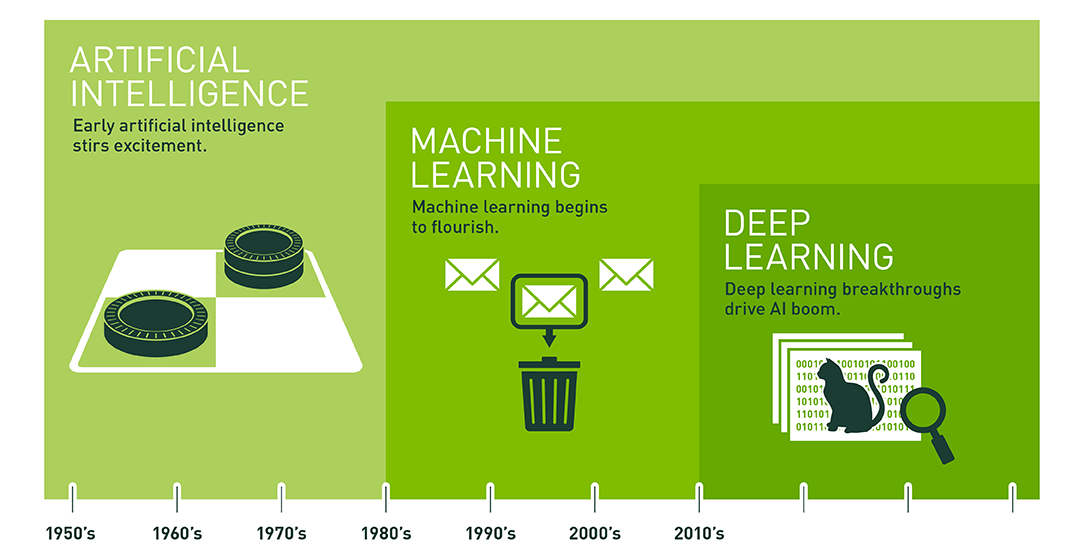
\includegraphics[width=\textwidth]{Deep_Learning_Icons_R5_PNG}
    \caption{\cite[page 5]{nvidia-ai-explained} Relationsship of AI, ML \& DL}
    \label{fig:ai_ml_dl_termns}
\end{figure}

Machine learning uses algorithms to parse data, learn from it and then make determinations or predictions.
In practice it is helping software to perform a result without the explicit programming of rules.
To be able to get answers from data using machine learning there are multiple steps involved:
\cite{nvidia-ai-explained, tensorflow-about}

\begin{figure}[H]
    \centering
    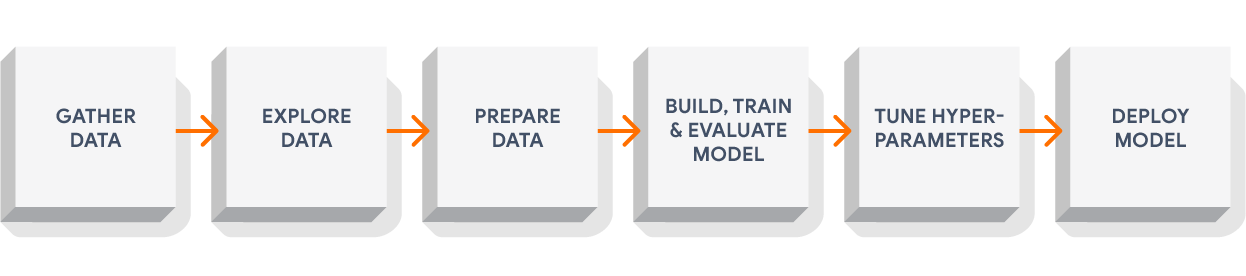
\includegraphics[width=\textwidth]{how_ml_works_tab2_graphic}
    \caption{\cite{tf_ml_steps_pipline} Steps to solving an machine learning problem}
    \label{fig:ml_steps_pipeline}
\end{figure}

In machine learning there are three main paradigms called supervised learning, unsupervised learning and reinforcement learning:

\begin{figure}[H]
    \centering
    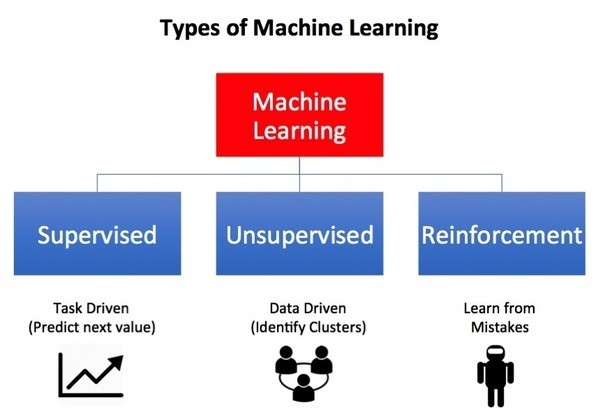
\includegraphics[width=\textwidth]{machine_learning_paradigms}
    \caption{\cite{ml_paradigms_image} Machine learning paradigms}
    \label{fig:ml_paradigms_image}
\end{figure}

In \textbf{supervised learning}, the network trains on a big dataset.
The dataset is composed of a lot of examples.
Each example has its correct result attached to it.
The examples are called features and their outcome is a label.
This approach is good for classification (categorial or discrete) and regression (numerical or continuous) problems.
\cite{nvidia_paradigms_blog}
\hfill \break
In contrast, \textbf{unsupervised learning} uses unlabelled data, because there is no desired outcome or correct answer.
The network tries to extract features and pattern on its own.
It can organize the data in different ways: clustering (separation of collections), anomaly detection, association
(feature correlation) and frequent pattern matching.
\cite{nvidia_paradigms_blog}
\hfill \break
In \textbf{reinforcement learning}, networks are agents and attempt to find the optimal way to accomplish a goal.
Agents are set on an environment, where the networks makes a decision.
An interpreter checks the decision and rewards or punishes the network.
This approach wants to find a long-term strategy and relies on learning from past feedback and exploration of new tactics.
\cite{nvidia_paradigms_blog}

Neural networks are inspired by the biology of a human brain.
A network consists of an input and output layer with at least one hidden layer.
Each layer is composed of nodes that are called neurons and connections between neurons which are called weights.
There are various differnet types of neural networks.
They differ based on their parameter representation and mathematical operations.
This article sticks with a classification of a deep neural network in a supervised learning manner.
The proposed technical approaches can be used with reinforcement learning as well.
Figure \ref{fig:dnn_1hidden_example} shows a fully connected neural network with one hidden layer:
\cite{nvidia-ai-explained, tensorflow-about}

\begin{figure}[H]
    \centering
    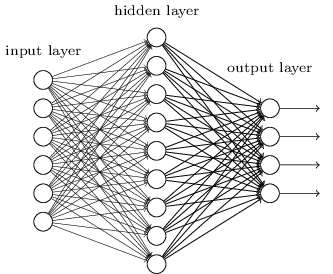
\includegraphics[scale=.6]{dnn_1hidden_example}
    \caption{\cite{dnn_1hidden_example_image} Example of a neural network}
    \label{fig:dnn_1hidden_example}
\end{figure}

To be abe to classify on data, the neural network has to be trained.
In the training phase "teaches" the network itself how to understand data by classifying records or making predictions. \cite{ibm-watson-healthcare}
The weights and neurons on each layer begin with random values which are improved over time to make the network more accurate.
In the training process a loss function quantifies how inaccurate the network is and a procedure called backpropagation is used to adjust each weight and neuron for an better accuracy.
\cite{nvidia-ai-explained, tensorflow-about}

\begin{figure}[H]
    \centering
    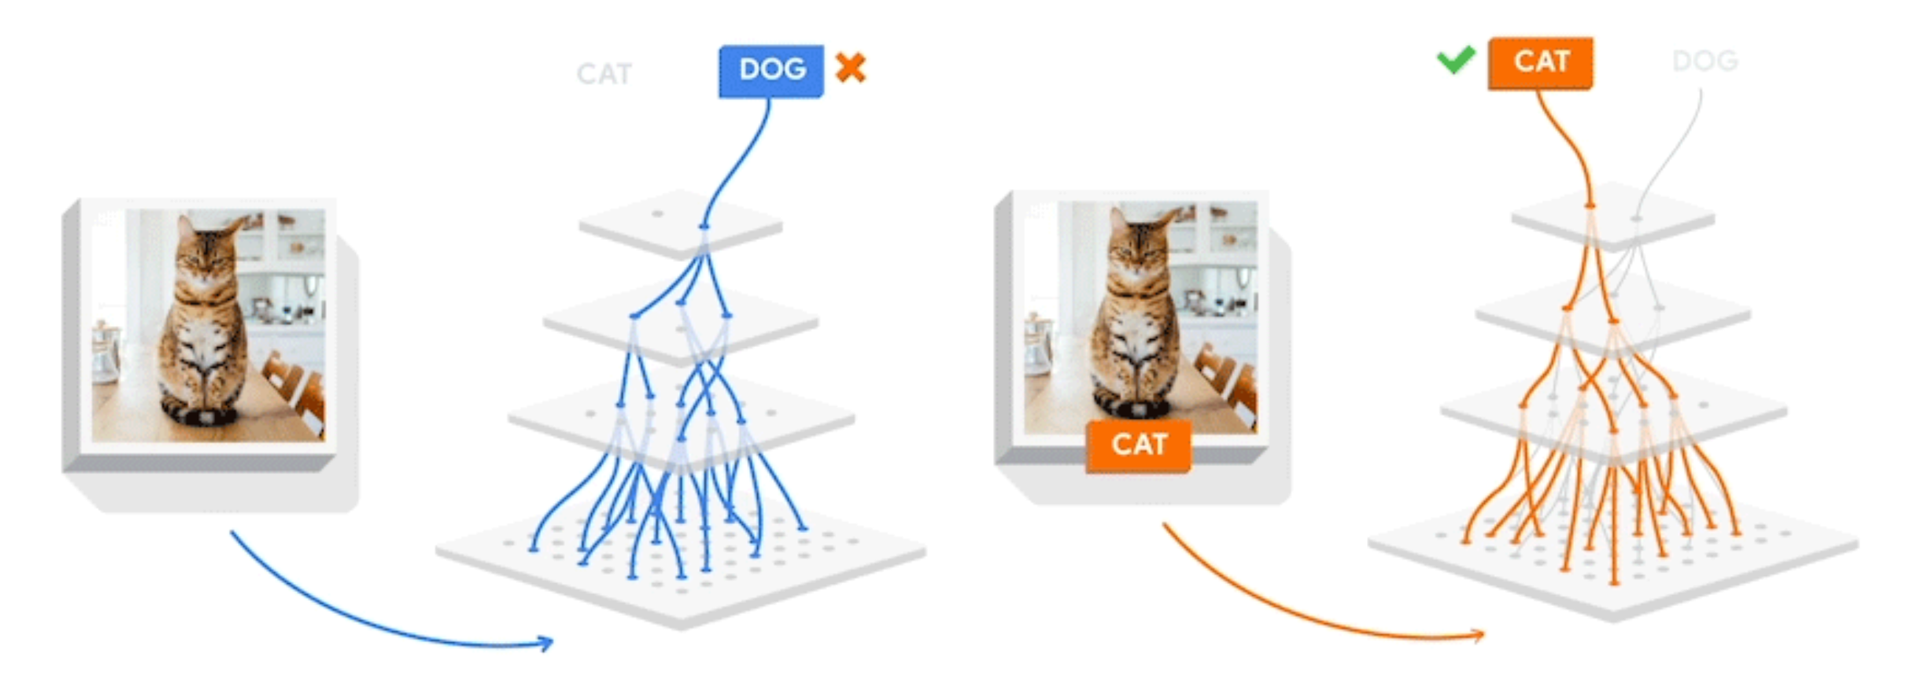
\includegraphics[width=\textwidth]{training-dnn-cat-example}
    \caption{\cite{tf_dnn_training_cat_example} Training of a neural network}
    \label{fig:tf_dnn_training_cat_example}
\end{figure}

The training result of a neural network is a model.
The model consists of all weight and neuron values.
\hfill \break
This model can predict all classifications it learned from the dataset.
A good representation for understanding the insight of a network is to take a closer look to the values each neuron stores.
Each neuron in the model learned an abstract representation of the data.
This results in a feature hierarchy between the different layers \cite{skymind_neural_network}.
Neurons on the first layers learn to detect lines from the input.
The layers after that learn combine the lines to shapes.
The last layers can recognize textures based on the shapes.
The textures together conclude to the final prediction.
Figure \ref{fig:tf_dnn_shapes_textures} shows a visual diagram of a network detecting lines, shapes, and textures:
\cite{nvidia-ai-explained, tensorflow-about}

\begin{figure}[H]
    \centering
    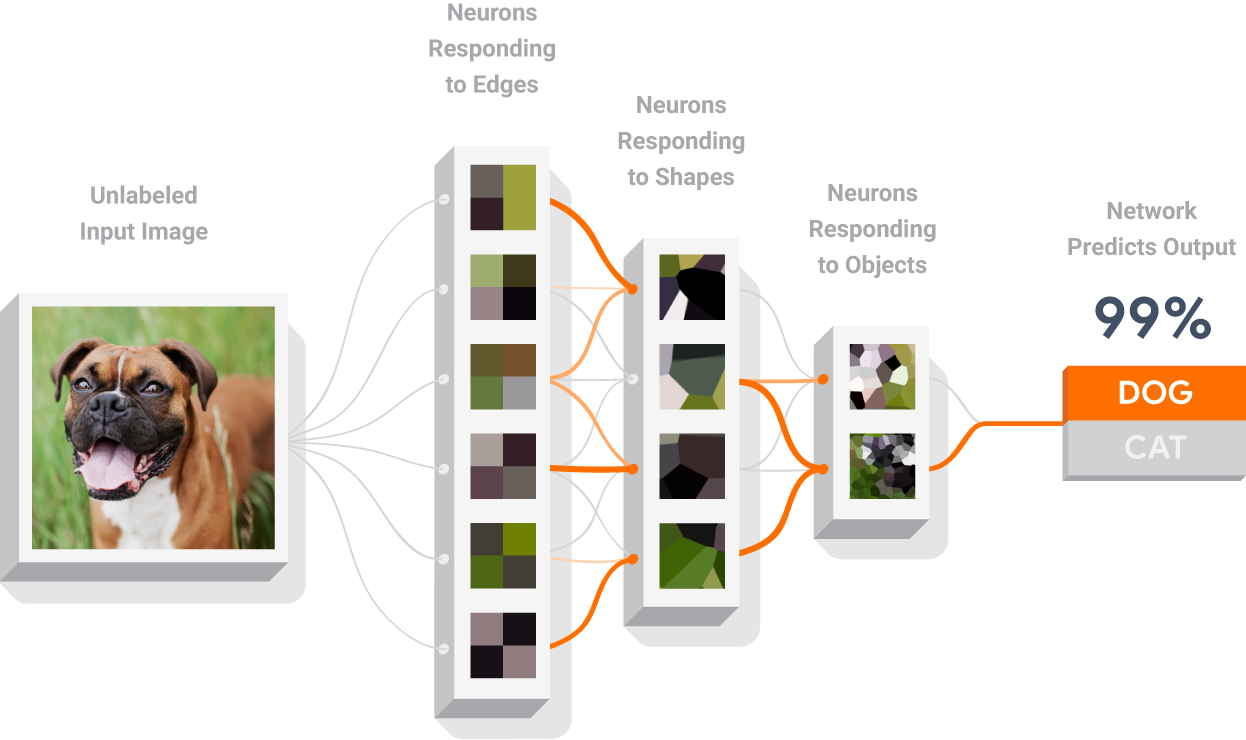
\includegraphics[width=\textwidth]{how_ml_works_tab3_graphic}
    \caption{\cite{tf_dnn_shapes_textures} Anatomy of a neural network}
    \label{fig:tf_dnn_shapes_textures}
\end{figure}

\section{Motivation}

These use-cases show great solutions for real-world problems solved with deep learning approaches.
However, current deep learning solutions are facing two major challenges:

AI is such a powerfull tool that more and more people are concerned about misuses of the technology.
Many people claim a governance of AI by governments and social guidelines.
An open letter with the title "Research priorities for robust and beneficial artificial intelligence" by the Future of Life institude is currently signed by over 8,000 artificial intelligence experts, researchers and successful businessmen \cite{futureoflife-ai-open-letter, futureoflife-research-priorities}.
The letter affirms a great potential of artificial intelligence for society, but calls for concrete research on: "…how to reap its benefits while avoiding potential pitfalls" \cite{futureoflife-ai-open-letter}.
Another example is a white paper published by Google with the title "Perspectives on Issues in AI Governance".
Google which provides on of the biggest ecosystems for machine learning as an open source platform shares their point of view in explainability standards, fairness appraisal, safety considerations, human-AI collaboration and liability frameworks with commentaries on the issues and suggestions of actions \cite{google-ai-governance}.
Moreover they invoke governments and civil society groups to contribute to the AI governance discussion.
According to Google there are already many regulations and legal codes that are broad enough to apply to AI and high level contentions by policymakers \cite[page 3]{google-ai-governance}.
Google acknowledges the first steps and hopes to help with their deeper insights for deeper discussions \cite[page 4]{google-ai-governance}.
\hfill \break
Besides the white paper they published their principles for using the technology.
They assess AI applications to be socially beneficial, avoiding unfair bias, built and tested for safety, are accountable to people, include privacy design principles, have high standards of scientific excellence and are made available for uses that concur with these principles.
In addition to their objectives for AI applications, they list areas where they will not design or deploy applications:
Technologies that cause harm, facilitate injury to people, violating internationally accepted norms or is against accepted principles of international law and human rights.
\cite{google-ai-principles}
\hfill \break
A similar approach has the German Telekom AG, one of the largest telecommunication providers in europe.
In November 2018 they shared their guidelines for artificial intelligence in a public blog post.
They take actions under their guidelines of transparency, security, responsibility and caring for the customer.
\cite{telekom-ai-guidelines}

The second obstacle is the ongoing improvement in machine learning:
\hfill \break
Deep learning techniques have been proven shining with a large number of labeled datasets and outperform many machine learning techniques.
With new attention to unsupervised and reinforement learning which are aiming to solve complex tasks without explicit knowledge improves the effort of creating datasets for training models \cite{continual-ai-blog, alphastar}.
However, most deep learning techniques are solving specific, isolated tasks which are not able to learn new tasks with a given model \cite{continual-ai-blog}.
Many real-world scenarios require the ability of multi-task learning.
Multi-task learning menas that deep neural networks are able to learn multiple consecutive tasks without forgetting previous tasks \cite{elastic-weight-consolidation}.
This challenge results in the paradigm of "continual learning".
Other common designations are "incremental learning", "continuous learning" or "lifelong learning" \cite{lifelong-machine-learning-book, continual-ai-blog}.
The oldest term is "lifelong learning" and was used in areas outside of deep learning \cite{continual-ai-blog}.
This is why there were the introduction of modern terms like "continuous" or "continual", which are targeting specifically deep learning algorithms.
\cite{continual-ai-blog}
The Oxford Dictionary says that "continuous" is five times more prominent than "continual" and refers to "no interruption". "Continual" on the other hand includes the meaning of "inbetween intervals" or "happening frequently".
\cite{oxford-continual-continuous}
The meaning of "Continual" is a closer definition to this article and will be used together with the term of "incremental", which is a more technical term for the domain.
\hfill \break

% aktueller approach
% mit bild untermauern
% auf probleme zu sprechen kommen und wie es aussehen sollte

% irgendwie die beiden unteren punte einbauen und auf general intelligence zu sprechen zu kommen
% what are more achievemnts:
% scale
% machine intelligence

% closer: that it is as important as reinforcement learning for a machine general intelligence

These ideas of continuously and adaptively learning about new features would enale an autonomous incremental development and the ability of learning more complex skills and knowledge.
\cite{continual-ai-blog}

One major step towards an artificial general intelligence or machine intelligence is the removing of the barrier which is called "catastrophic forgetting".
% Um dies zu erreichen muss die techbologie zuerst die große Hürde des catastrophic forgetting beseitigen.

% touch the big problem big problem: catastrophic forgetting
% first solution tries with algorithms

% great use-case that touches both challenges

\section{Related Work}


\subsection*{Better Weight Consolidation}

This paper proposes an improvement of the Elastic Weiht Consolidation. They specifically address the diagonal assumption made by the EWC algorithm.

https://arxiv.org/pdf/1802.02950.pdf


\section{Project Introduction}

… % TODO
% the first dolution tries use all one fisher matrix
% calculation takes a lot of time
% idea of optimizing the algorithms with a adjustment of the matrix

% the goal to optimize these algorithms that they may be used in real-world scenarios